\documentclass{exam}

\pagenumbering{gobble}
\usepackage{graphicx} %for graphix
\usepackage{titling}
\setlength{\droptitle}{-8ex}
\pretitle{\begin{flushleft}\Large\bfseries}
\posttitle{\par\end{flushleft}}
\preauthor{\begin{flushleft}\Large}
\postauthor{\end{flushleft}}
\predate{\begin{flushleft}}
\postdate{\end{flushleft}}
\usepackage{enumerate} %for alphabetized lists
\usepackage{amsmath}
\usepackage{multicol} %for multiple columns
\usepackage{systeme} %systems of equations
\renewcommand{\questionshook}{\setlength{\itemsep}{15pt}} %controls space betweenites

%fromhttps://texblog.org/2012/06/25/adding--lines--for--taking--handwritten--notes--in--latex/
\usepackage{pgffor, ifthen}
\newcommand{\notes}[3][\empty]{%q
   vspace{10pt}\\
    \foreach \n in {1,...,#2}{%
        \ifthenelse{\equal{#1}{\empty}}
            {\rule{#3}{0.5pt}\\}
            {\rule{#3}{0.5pt}\vspace{#1}\\} 
        }
}

\title{Problem set \#7}

\author{ \textbf{Name: }  \enspace\hrulefill \\ Precalculus \\ Herbert H. Lehman High School } 


\begin{document}
\maketitle
\thispagestyle{empty}


\noindent The marketing department at \textbf{Jada$^2$ Inc.}  has suggested that the company's trail mix products standardize on every mix being one-third peanuts. Adjusting the peanut portion of each recipe by also adjusting the chocolate portion leads to revised recipes,  as given in the following table:


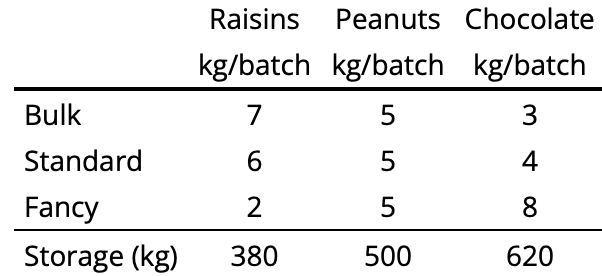
\includegraphics[scale=0.5]{table.png}

\noindent The production manager insists that enough of each mix should be made so that no ingredients are left over at the end of the day. \textbf{Your job is to write a report  determining how much of each mix should be made, so that both the marketing department and the production manager are happy.} Use the questions below to guide your writing of the report.
\begin{questions}

\question 
\begin{parts}
\part
Write an \textbf{$AX=B$} matrix equation to represent the information in the table, using $b$, $s$, and $f$ to represent the number of batches in the bulk, standard, and fancy mix.
\part
Find the adjugate and determinant for A (feel free to use the calculators on Google Classroom!)
\part 
If possible, use the adjugate and determinant to find the inverse $A^{-1}$. If not, explain why you cannot find it in a complete sentence
\part What do you think this tells you about the problem you're trying to solve?
\end{parts}
\question 
\begin{parts}
\part Determine if your  \textbf{$AX=B$} matrix equation  has one solution, no solution, or infinitely many solutions.  
\part If possible, find \textbf{at least one solution} that works for  \textbf{$AX=B$} matrix equation
\end{parts}
\question 
 \textbf{write a paragraph responding to the marketing department's suggestion while also making the production manager happy}. Be sure to reference your findings from (1) and (2) to support your response!
\end{questions}



\end{document}